\definecolor{myblue}{RGB}{56,94,101}

\begin{figure}
   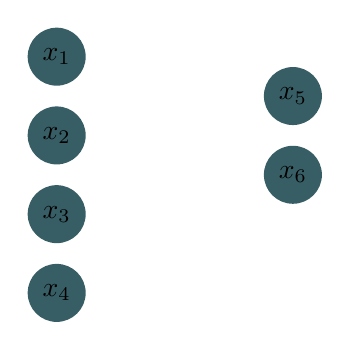
\begin{tikzpicture}[arrow/.style={thick,->,black},
            set name/.style={font=\color{myblue}\tiny\bfseries\sf},
            set/.style={ultra thick, myblue},
            every node/.style={circle},
            font=\sf
         ]
      \node[fill=myblue] (x1) at (1.0, 3.0) {$x_1$};
      \node[fill=myblue] (x2) at (1.0, 2.0) {$x_2$};
      \node[fill=myblue] (x3) at (1.0, 1.0) {$x_3$};
      \node[fill=myblue] (x4) at (1.0, 0.0) {$x_4$};
      \node[fill=myblue] (x5) at (4.0, 2.5) {$x_5$};
      \node[fill=myblue] (x6) at (4.0, 1.5) {$x_6$};


   \end{tikzpicture}
\end{figure}